%Example of use of oxmathproblems latex class for problem sheets
\documentclass{oxmathproblems}
\usepackage{hyperref}
%(un)comment this line to enable/disable output of any solutions in the file
%\printanswers
%define the page header/title info
\course{Algorithm Design and Analysis}
\sheettitle{Assignment 1 \\ Deadline: March 24, 2024} %can leave out if no title per sheet
\begin{document}
\begin{questions}
\miquestion[25]
Asymptotic notations.
\begin{parts}
    \part In each of the following situations, indicate whether $f=O(g)$, or $f=\Omega(g)$, or both (in which case $f=\Theta(g)$). Justify your answer.
    \begin{enumerate}
        \item $f(n)=n^{1/2}$ and $g(n)=5^{\log_2n}$
        \item $f(n)=100n+\log n$ and $g(n)=n+(\log n)^2$
        \item $f(n)=(\log n)^{\log n}$ and $g(n)=n/\log n$
        \item $f(n)=(\log n)^{\log n}$ and $g(n)=2^{(\log_2n)^2}$
        \item $f(n)=\sum_{i=1}^ni^k$ and $g(n)=n^{k+1}$
    \end{enumerate}
    \part Let $f(n)=\left(2\cdot \lceil \frac n2\rceil\right)!$ and $g(n)=\left(2\cdot \lfloor \frac n2\rfloor+1\right)!$. Prove that neither $f=O(g)$ nor $f=\Omega(g)$ is true.
\end{parts}
Answer:
\begin{parts}
    \part
        \begin{enumerate}
            \item $f(n)=O(g)$\newline
            \proofname:According to \textit{Change of Base Formula},$g(n)=n^{\log_25}$,which is strictly greater than $f(n)$ over the interval from 0 to positive infinity,so we can infer from the definition that $f(n)=O(g)$.
            \item $f(n)=\Theta(g)$\newline
            \proofname:Based on the properties of the logarithmic function,$\log n=o(n)$,so is $(\log n)^2$,in that case,we can easily figure out that 
            $\lim_{n\to\infty}\frac{f(n)}{g(n)}=100$.Based on the asymptotic theorems for functions,we have $f(n)=\Theta(g)$.
            \item $f(n)=\Omega(g)$\newline
            \proofname:According to \textit{Change of Base Formula},$f(n)=n^{\log{\log n}}$,which is obviously greater than $g(n)$ when $n$ is large enough,so we
            can conclude that  $f(n)=\Omega(g)$.
            \item $f(n)=O(g)$\newline
            \proofname:After calculation,$f(n)=n^{\log{\log n}}$,$g(n)=n^{\log_2n}$.Because
            of $\log{\log n} = o(\log_2n)$,we know $f(n)=O(g)$.
            \item $f(n)=\Theta(g)$\newline
            \proofname:Here we give the recurrence formula without proof,$S_k(n)=\frac{n^{k+1}}{k+1}-\frac{1}{k+1} \sum_{i=0}^{k-1}(-1)^{k-i}\binom{k+1}{i} S_i(n)$,in which $S_k(n)=\sum_{i=1}^{n}i^k$,therefore,the functions above satisfy $f(n)=\Theta(g)=\Theta(n^{k+1})$.
        \end{enumerate}
    \part   By definition,if n is even,then there would be 
            $\lceil \frac{n}{2}\rceil = \lfloor \frac{n}{2}\rfloor = \frac{n}{2}$.In that case ,$f(n)=n!$ and $g(n)=(n+1)!$ apparently satisfy $f=O(g)$.Similarly,if n is odd,then $f(n)=(n+1)!$,$g(n)=n!$,in which $f=\Omega(g)$.While $n$
            is random,neither $f=O(g)$ nor $f=\Omega(g)$ is absolutely true.
\end{parts}
\miquestion[25]
Prove the following generalization of the master theorem. Given constants $a\geq 1,b> 1,d\geq 0$, and $w\geq 0$, if $T(n)=1$ for $n<b$ and $T(n) = aT(n/b) + n^d\log^w n$, we have
  $$
    T(n) = \begin{cases}
      O(n^d\log^w n) & \mbox{if }a < b^d \\
      O(n^{\log_b a}) & \mbox{if }a > b^d \\
      O(n^d\log^{w+1} n) & \mbox{if }a = b^d
    \end{cases}.
  $$
Answer:\newline
Let us say that $n=b^k$ and $f(n)=n^d\log^{\omega}n$,After iteration we can get
\begin{equation}
    T(n)=c_1n^{\log_b a}+\sum_{j=0}^{k-1}{a^j f(\frac{n}{b^j})}
\end{equation}
\begin{parts}
    \part   if $a < b^d$,$af(\frac{n}{b})\leq cf(n)$,so
            \begin{align}
            &T(n)\leq c_1n^{\log_b a}+\sum_{j=0}^{log_b n-1}c^jf(n)\\
            &=c_1n^{\log_b a}+f(n)\frac{c^{{\log_b n}-1}}{c-1}\\
            &=c_1n^{\log_b a}+\Theta(f(n))
            \end{align}
            Besides,$T(n)\geq f(n)$,therefore,$T(n)=O(n^d\log^w n)$.
    \part   if $a > b^d$,$f(n)=O(n^{{\log_b a}-\epsilon})$
            \begin{align}
            &T(n)=c_1n^{\log_b a}+O(\sum_{j=0}^{log_b n-1}{a^j (\frac{n}{b^j}})^{{{log_b a}}-\epsilon})\\
            &=c_1n^{\log_b a}+O(n^{{{log_b a}}-\epsilon}\sum_{j=0}^{log_b n-1}{\frac{a^j}{(b^{{log_b a}-\epsilon})^j}})\\
            &=c_1n^{\log_b a}+O(n^{{{log_b a}}-\epsilon}\frac{b^{\epsilon{log_b n}-1}}{b^\epsilon -1})\\
            &=c_1n^{\log_b a}+O(n^{{{log_b a}}-\epsilon}n^\epsilon)\\
            &=O(n^{log_b a})
            \end{align}
    \part   if $a = b^d$,$f(n)=\Theta(n^{\log_b a}\log^w n)$
            \begin{align}
            &T(n)=c_1n^{\log_b a}+\Theta(\sum_{j=0}^{log_b n-1}{a^j (\frac{n}{b^j}})^{log_b a}\log^w n)\\
            &=c_1n^{\log_b a}+\Theta(n^{log_b a}logn\log^w n)\\
            &=\Theta(n^{log_b a}log^{w+1}n)=O(n^d\log^{w+1} n)
            \end{align}
\end{parts}
\miquestion[25]
Given an array $A[1\cdots n]$ of integers, a pair of indices $(i,j)$ is an \emph{inversion} if $i<j$ and $A[i]>A[j]$.
Design an algorithm that counts the number of inversions in $O(n\log n)$ time.
\textbf{Hint:} Suppose the first half of the array $A[1\cdots (n/2)]$ and the second half of the array $A[(n/2+1)\cdots n]$ (say, $n$ is an even number) are sorted by ascending order, can you count the number of inversions in $O(n)$ time?\newline
Answer:
\begin{parts}
    \part Split the array into two parts, recursively sort the left and right halves separately, while keeping track of the number of inversions.
    \part When merging two sorted subarrays, simultaneously count the number of inversions across the two subarrays. Since the two subarrays are already sorted, it is possible to count the number of inversions in linear time during the merging process.
    \part Return the total number of inversions counted during the recursive sorting process.
    \begin{figure}[htb]
    \centering
    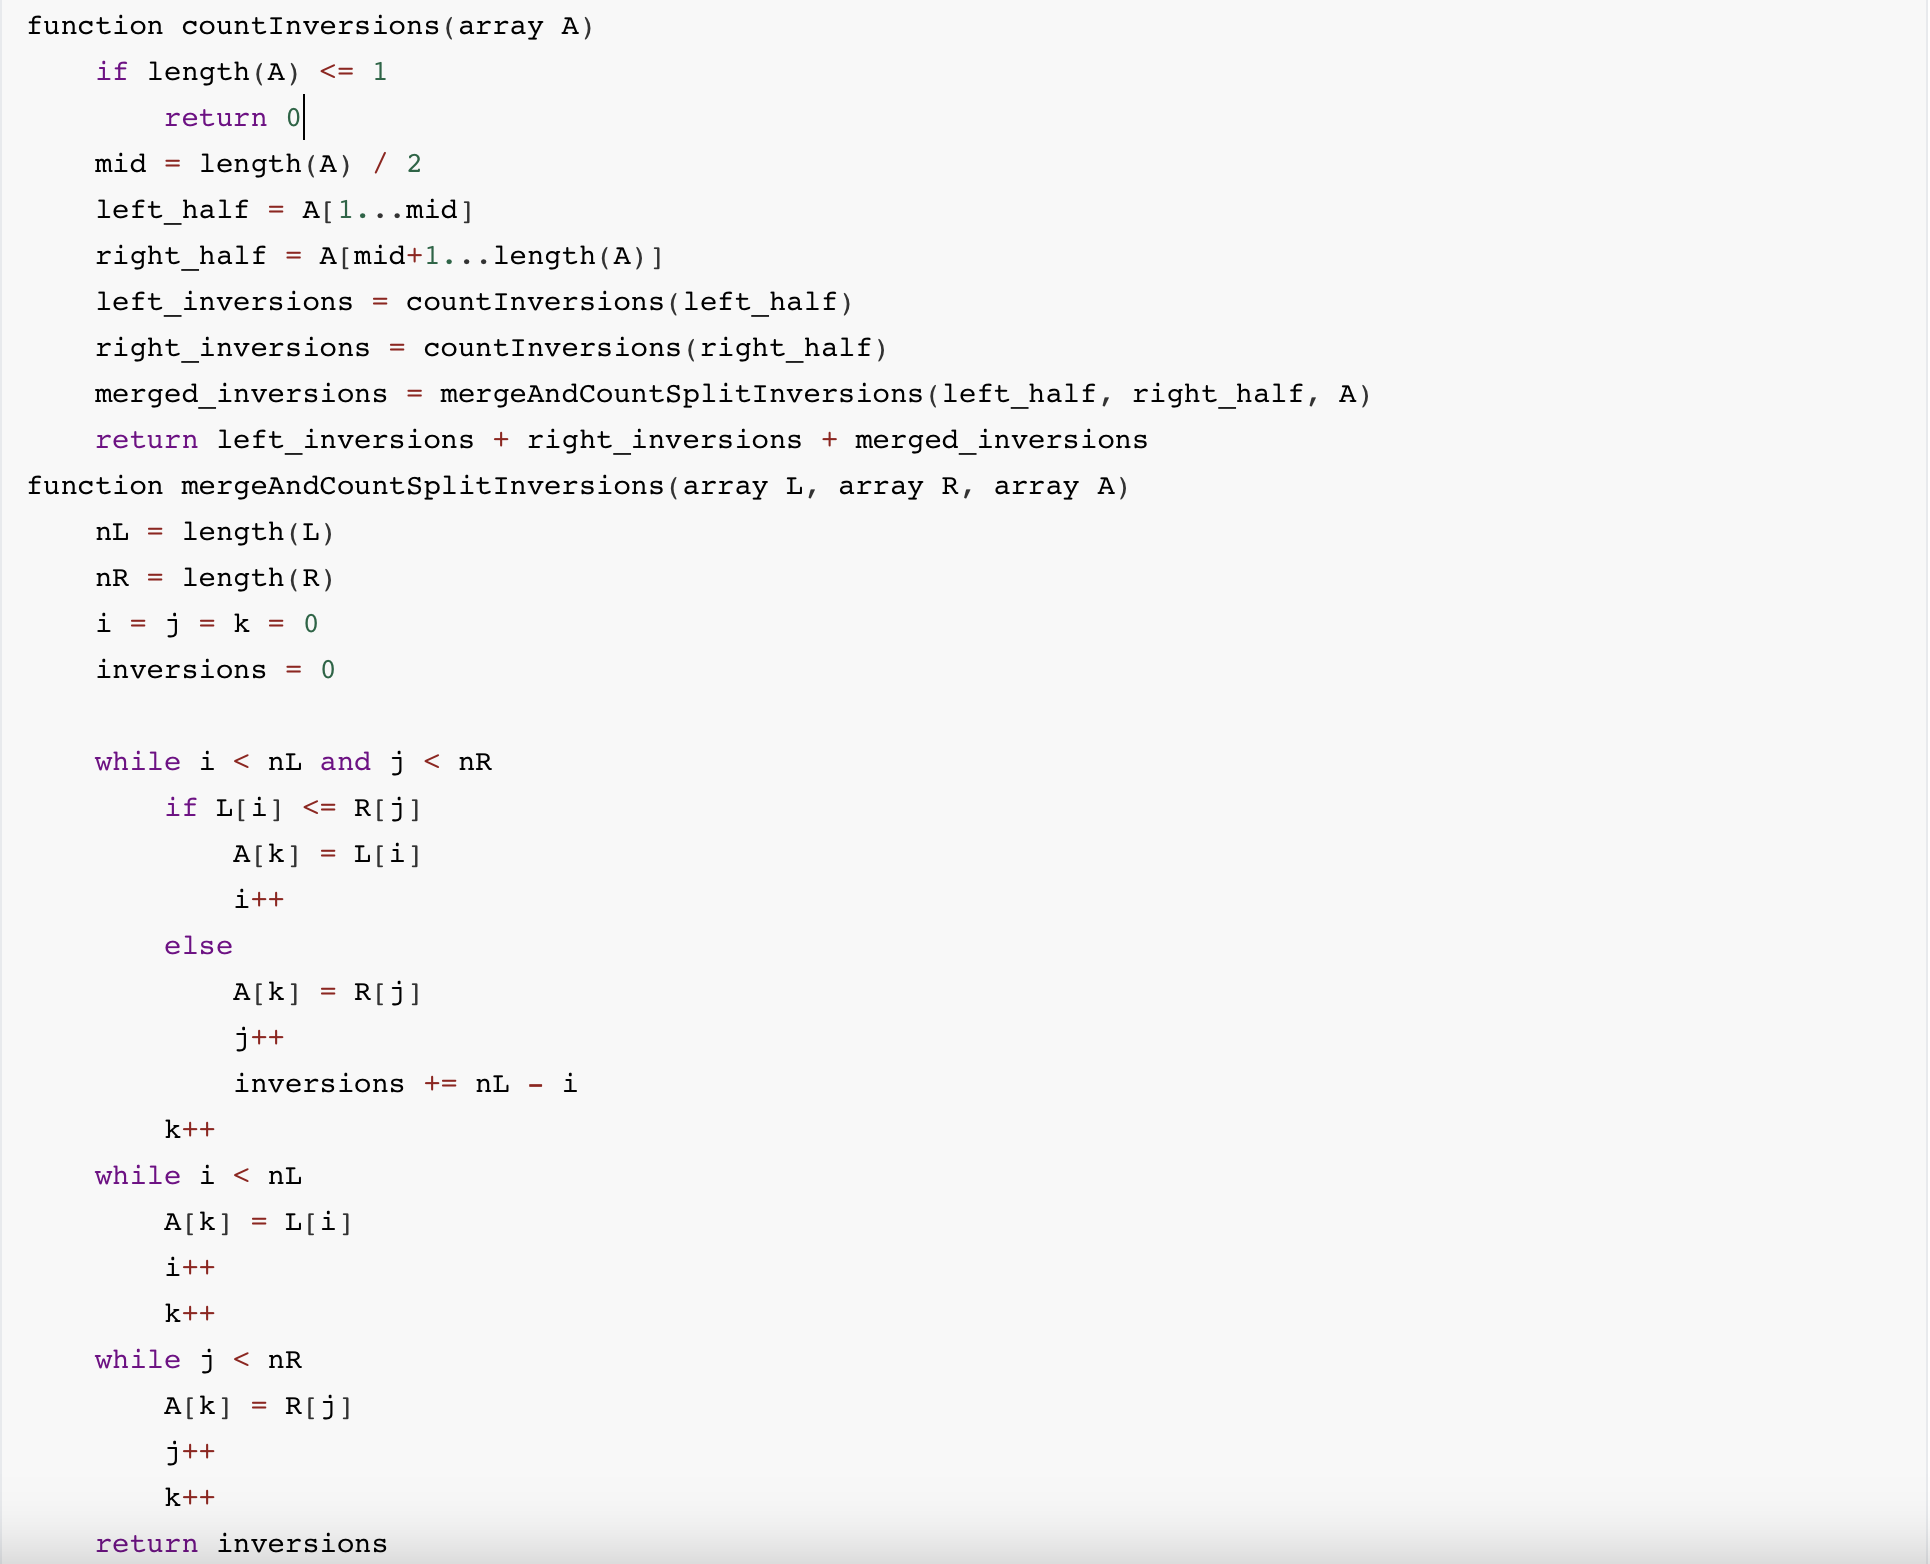
\includegraphics[width=.9\linewidth]{hw1/3.1.png}  
    \caption{Algorithm pseudocode}
    \label{fig}
    \end{figure}
\newline
Suppose the array A is divided into two sorted halves, left[1..n/2] and right[(n/2+1)..n], where n is even.\\

1.Initialize count = 0, to accumulate the number of inversions.\\
2.Use two pointers i and j, pointing to the start of left and right arrays, respectively.\\
3.Compare left[i] and right[j]:\\
a) If left[i] $<=$ right[j], then left[i] is not an inversion with any element in the right array, so increment i.\\
b) If left[i] $>$ right[j], then left[i] forms an inversion with all elements from right[j] to the end of the right array. Increment count by (right.length - j + 1), and increment j.\\
4.Repeat step 3 until either i or j reaches the end of their respective arrays.\\
5.The final value of count is the number of inversions between the left and right halves.\\
Since left and right are already sorted, an element in left can only form inversions with elements larger than itself in the right array. We only need to consider the number of elements in the right array that are smaller than the current element in the left array.The time complexity of this process is O(n) because the pointers i and j traverse the left and right arrays only once, regardless of the number of inversions.Therefore, given the two sorted halves of the array, we can count the inversions between them in linear time.
\end{parts}
\miquestion[25]
Let $A$ be a square matrix. This question discusses the computation of $A^2$.
\begin{parts}
    \part Show that five multiplications are sufficient to compute the square of a $2\times 2$ matrix.
    \part What is wrong with the following algorithm for computing the square of an $n\times n$ matrix?
    \begin{itemize}
        \item Use a divide-and-conquer approach as in Strassen's algorithm, except that instead of getting $7$ subproblems of size $n/2$, we now get $5$ subproblems of size $n/2$ thanks to part (a). Using the same analysis as in Strassen's algorithm, we can conclude that the algorithm runs in time $O(n^{\log_25})$.
    \end{itemize}
    \part In fact, squaring matrices is no easier than matrix multiplication. In this part, you will show that if $n\times n$ matrices can be squared in time $S(n)=O(n^c)$, then any two $n\times n$ matrices can be multiplied in time $O(n^c)$.
    \begin{enumerate}
        \item Given two $n\times n$ matrices $A$ and $B$, show that the matrix $AB+BA$ can be computed in time $3S(n)+O(n^2)$.
        \item Given two $n\times n$ matrices $X$ and $Y$, define the $2n\times 2n$ matrices $A$ and $B$ as follows:
        $$A=\left[\begin{array}{cc}
            X & 0 \\
            0 & 0
        \end{array}\right]\qquad\mbox{and}\qquad B=\left[\begin{array}{cc}
            0 & Y \\
            0 & 0
        \end{array}\right].$$
        What is $AB+BA$, in terms of $X$ and $Y$?
        \item Using 1 and 2, argue that the product $XY$ can be computed in time $3S(2n)+O(n^2)$. Conclude that matrix multiplication takes time $O(n^c)$.
    \end{enumerate}
\end{parts}
Answer:
\begin{parts}
    \part   
    Let A be a 2×2 matrix represented as:
    $$\begin{bmatrix}
    a&b\\
    c&d\\
    \end{bmatrix}$$
    we can reduce the number of multiplications to 5 by using the following strategy:
    \begin{enumerate}
        \item Compute p = $a^2$
        \item Compute q = $d^2$
        \item Compute r = $bc$
        \item Compute s = $b(a+d)$
        \item Compute t = $c(a+d)$
    \end{enumerate}
    then we can compute $A^2$ as:
    $$\begin{bmatrix}
    p+r&s\\
    t&q+r
    \end{bmatrix}
    $$
    \part
    Because of the difference between matrix multiplication and number
    multiplication,for example,$(AB+BD)\neq B(A+D)$,we can't divide the original problem into 5 subproblems of the same type.Besides,
    the cost of matrix multiplication is not accordant to squaring matrices when we discuss $2\times 2$ matrix.Hence the recurrence $T (n) = 5T (n/2) + O(n^2)$ does not make sense.
    \part
    \begin{enumerate}
        \item We can compute the matrix $AB+BA$ by computing $(A+B)^2-A^2-B^2$ which requires three squaring matrices,costing time $3S(n)$.Besides,adding $n \times n$ matrices cost $n^2$ every time.As $n\times n$ matrices can be squared in time $S(n)$,the matrix $AB+BA$ can be computed in time $3S(n)+O(n^2)$.\\
        I'm curious about whether the method below is correct:\\
        \textbf{We can compute the matrix $AB+BA$ by computing $\frac{(A+B)^2-(A-B)^2}{2}$ which requires two squaring matrices,costing time $2S(n)$.Considering the addition time, we can compute the matrix $AB+BA$ in time $2S(n)+O(n^2)$.}

        \item 
        $$AB=\left[\begin{array}{cc}
            0 & XY \\
            0 & 0
        \end{array}\right]\qquad\mbox{and}\qquad BA=\left[\begin{array}{cc}
            0 & 0 \\
            0 & 0
        \end{array}\right].$$
        \item Given two $n\times n$ matrices $X$ and $Y$,we can
        use the matrices $A$ and $B$ to compute the $XY$ by computing $AB+BA$ which needs $3S(2n)+O(n^2)$ as discussed above.So for every matrix multiplication we can apply this trick to compute in time $O(n^c)$.Besides,we can define matrix $A$ below to enhance our conclusion.
        $$A=\left[\begin{array}{cc}
            0 & X \\
            Y & 0
        \end{array}\right]\qquad\mbox{and}\qquad A^2=\left[\begin{array}{cc}
            XY & 0 \\
            0 & YX
        \end{array}\right].$$
        Hence,it now suffices to compute $A^2$,as its upper left block will contain $XY$.The product can be calculated in time $O(S(2n))$.If $S(n)=O(n^c)$,this is also $O(n^c)$.
    \end{enumerate}
\end{parts}

\miquestion
How long does it take you to finish the assignment (including thinking and discussion)?
Give a score (1,2,3,4,5) to the difficulty.
Do you have any collaborators?
Please write down their names here.\newline
It takes me approximately 6 hours to finish the assignment.For my part,the difficulty is suitable as typing formula in latex takes up most of the time.Indeed,I encountered problems when solving \textbf{1.(a).5 and 4}.Here are references which helped me a lot:\\
\href{https://www.cnblogs.com/mdntct/p/17478419.html}{https://www.cnblogs.com/mdntct/p/17478419.html}\\
\href{https://stackoverflow.com/questions/27543250/whats-wrong-with-strassens-method-to-compute-square-of-a-matrix}{https://stackoverflow.com/questions/27543250/whats-wrong-with-strassens-method-to-compute-square-of-a-matrix}\\
Sadly,I'm not proficient in using latex,which causes some inaesthetics in presenting codes and urls.Wish your forgiveness and reviews!

\end{questions}
\end{document}
